\section*{Введение}

% На данный момент в программных системах самым распространенным представлением информации, которая создается пользователем или демонстрируется ему, является текстовое представление. Оно удобно по многим причинам, но у него есть существенный недостаток - часто без дополнительного стилизирования текстовая информация слишком тяжело воспринимается. При отображении данных для пользователя необходимо явственным образом сохранять изначальную структуру информации. В большинстве случаев такое стилизирование сводится к форматированию текста, то есть добавлению или удалению не несущих информацию символов, другому преобразованию текста без изменения его семантики. Данное преобразование называется \textbf{pretty printing}.

С появлением первых языков программирования особую важность приобрели языковые процессоры. \textbf{Языковой процессор} (\textbf{ЯП}) -- это программное средство, принимающее на вход текст на некотором языке (программирования, разметки и т. д.) и решающее определенную задачу над этим текстом. Языковые процессоры применяются для:
\begin{enumerate}
\item компиляции;
\item суперкомпиляции;
\item интерпретации;
\item статического анализа кода;
\item трансляции;
\item декомпиляции;
\item рефакторинга;
\item реинжиниринга.
\end{enumerate}
Также используются в средствах интегрированной разработки программного обеспечения. 

Первым этапом работы ЯП является \textbf{синтаксический анализ}, то есть сопоставление входного текста (линейной последовательности лексем) с формальной грамматикой языка. В результате работы синтаксического анализатора ЯП получает древовидное представление программы, над которым потом происходит основная работа.

Достаточно часто возникает задача показать пользователю промежуточный или конечный результат обработки кода.
А значит необходимо вернуться к текстовому представлению программы, то есть провести процедуру, обратную синтаксическому анализу. Такая задача называется \textbf{pretty printing}, а соответсвующий инструмент -- \textbf{pretty printer}.

Одной из проблем, возникающей при разработке pretty printer, является то, что непонятны и расплывчаты критерии результата работы pretty printer.
Очевидно, что одного соответствия с точки зрения синтаксиса и семантики полученного кода и древовидного представления недостаточно. Рассмотрим программы на рисунках~\ref{fig:wikiExUnfor} и \ref{fig:wikiExBSD}.

\begin{figure}[h!]
	\centering
	\inputminted{c}{codes/wikiExUnfor.c}
	\caption{Плохо отформатированный код}
	\label{fig:wikiExUnfor}
\end{figure}

\begin{figure}[h!]
	\centering
	\inputminted{c}{codes/wikiExBSD.c}
	\caption{Хорошо отформатированный код}
	\label{fig:wikiExBSD}
\end{figure}

Они эквиваленты синтаксически и семантически с точки зрения компилятора C, но для пользователя вариант с рисунка~\ref{fig:wikiExBSD} предпочтительней, так как надо приложить гораздо меньше усилий для его осознания. Как мы видим, при отображении данных необходимо явным для пользователя образом сохранять изначальную структуру информации. В большинстве случаев решение этой задачи сводится к добавлению или удалению символов, не несущих информацию для синтаксического анализа, другому преобразованию текста без изменения его семантики.

Кроме того определенную сложность в описание и исполнение конкретного pretty printer вносит тот факт, что в большинстве случаев нельзя однозначным образом сопоставить синтаксическую конструкцию с единственным шаблоном. Необходима вариативность в зависимости от дополнительных условий, наложенных на pretty printer.

Рассмотрим небольшой пример. Пользователь задает условие вида: “последовательные операторы пишутся на одной строке, если помешаются в N символов. Иначе - на разных строках”.

\begin{figure}[h]
	\centering
	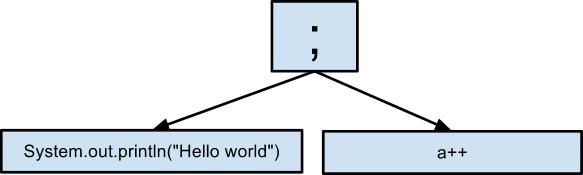
\includegraphics[width=0.8\textwidth]{seqTree}
	\caption{Последовательные операторы}
	\label{fig:seqImage}
\end{figure}

На рисунке~\ref{fig:seqImage} изображено синтаксическое дерево последовательности двух операторов. Такое дерево, согласно заданному правилу, может быть напечатано одним из двух вариантов (рисунки ~\ref{fig:seqCode1}, ~\ref{fig:seqCode2}).

\begin{figure}[h]
	\inputminted{c}{codes/seqCode1.java}
	\caption{Последовательные операторы. В строчку}
	\label{fig:seqCode1}
\end{figure}

\begin{figure}[h]
	\inputminted{c}{codes/seqCode2.java}
	\caption{Последовательные операторы. В несколько строк}
	\label{fig:seqCode2}
\end{figure}

Выбор происходит в зависимости от ширины вывода. Так при ширине равной 35 символов (длина строки “System.out.println(“Hello world”); ”), должен выбираться вариант, изображенный на рисунке~\ref{fig:seqCode2}, так как код на рисунке~\ref{fig:seqCode1} имеет ширину более 35 символов.
Могут быть заданы и более сложные условия.

\newpage

Рассмотрим другой пример. Пусть нам нужно текстовое представление синтаксического дерева конструкции If, и заданы шаблоны c рисунков~\ref{fig:ifTemplate1} и \ref{fig:ifTemplate2}.

\begin{figure}[h]
	\inputminted{haskell}{codes/ifTemplate1.hs}
	\caption{}
	\label{fig:ifTemplate1}
\end{figure}

\begin{figure}[h]
	\inputminted{haskell}{codes/ifTemplate2.hs}
	\caption{}
	\label{fig:ifTemplate2}
\end{figure}

Причем вариант, изображенный на рисунке~\ref{fig:ifTemplate1} выбирается в случае, если условие и ветки могут быть напечатаны в одну строчку. Тогда для деревьев, представленных на рисунках \ref{fig:ifImage1} и \ref{fig:ifImage2}, будут напечатаны коды с рисунков \ref{fig:ifCode1} и \ref{fig:ifCode2} соответственно.

\begin{figure}[h!]
	\begin{minipage}[b]{0.65\linewidth}
		\centering
		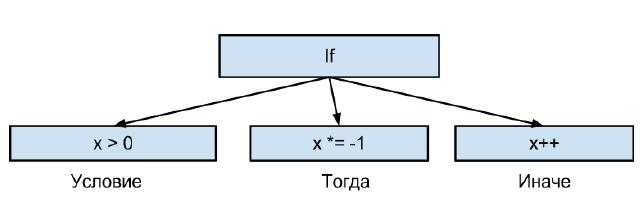
\includegraphics[width=\textwidth]{if1}
		\caption{}
		\label{fig:ifImage1}
	\end{minipage}
	\hspace{0.5cm}
	\begin{minipage}[b]{0.25\linewidth}
		\centering
		\inputminted{haskell}{codes/ifCode1.hs}
		\caption{}
		\label{fig:ifCode1}
	\end{minipage}
\end{figure}

\begin{figure}[h!]
	\begin{minipage}[b]{0.65\linewidth}
		\centering
		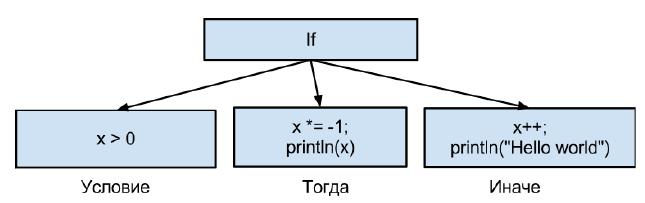
\includegraphics[width=\textwidth]{if2}
		\caption{asd}
		\label{fig:ifImage2}
	\end{minipage}
	\hspace{0.5cm}
	\begin{minipage}[b]{0.25\linewidth}
		\centering
		\inputminted{haskell}{codes/ifCode2.hs}
		\caption{}
		\label{fig:ifCode2}
	\end{minipage}
\end{figure}

% Постановка задачи
То, что не существует четких критериев красоты кода, и отсутствие библиотек, предоставляющих возможность описать pretty printer в виде, подобном
рассмотренному примеру с конструкцией If, то есть с помощью шаблонов, часто приводит к тому, что pretty printer становятся крайне сложными и наполненными эвристиками.

Задачей данной работы было рассмотреть возможность определения pretty printer с помощью шаблонов, при условии, что существует расширяемый синтаксический анализатор для целевого языка.